\subsection{Aufgabenstellung}
Das Ergebnis des Projekts Edubot soll ein simpel zu bedienendes, funktionales und effektives Werkzeug zum Erlernen der grundsätzlichen Arbeitsweise eines Roboters darstellen. Es soll im Anschluss an diese Diplomarbeit im Fach “Prozessregelung mit Laborübungen” verwendet werden. Das Projekt beinhaltet eine Programmierschnittstelle (API) mit der  Schüler den Roboter schnell und einfach in ihre eigenen Programme einbinden können, sowie eine Endanwendung welche zu Präsentations- und Unterrichtszwecken verwendet werden kann.
\\[0.5em]
Zusätzlich zu den erwähnten Funktionen soll ein ausführliches Dokumentations und Hilfesystem m zur Verfügung gestellt werden, um es dem Anwender zu ermöglichen, sowohl die Funktionen der API zu verstehen, als auch einen Einblick in die Funktionsweise der Anwendung und der Hardware zu erlangen.
\\[0.5em]

\begin{figure}[H]
  \centering
  \begin{minipage}[t]{12 cm}
  	\centering
  	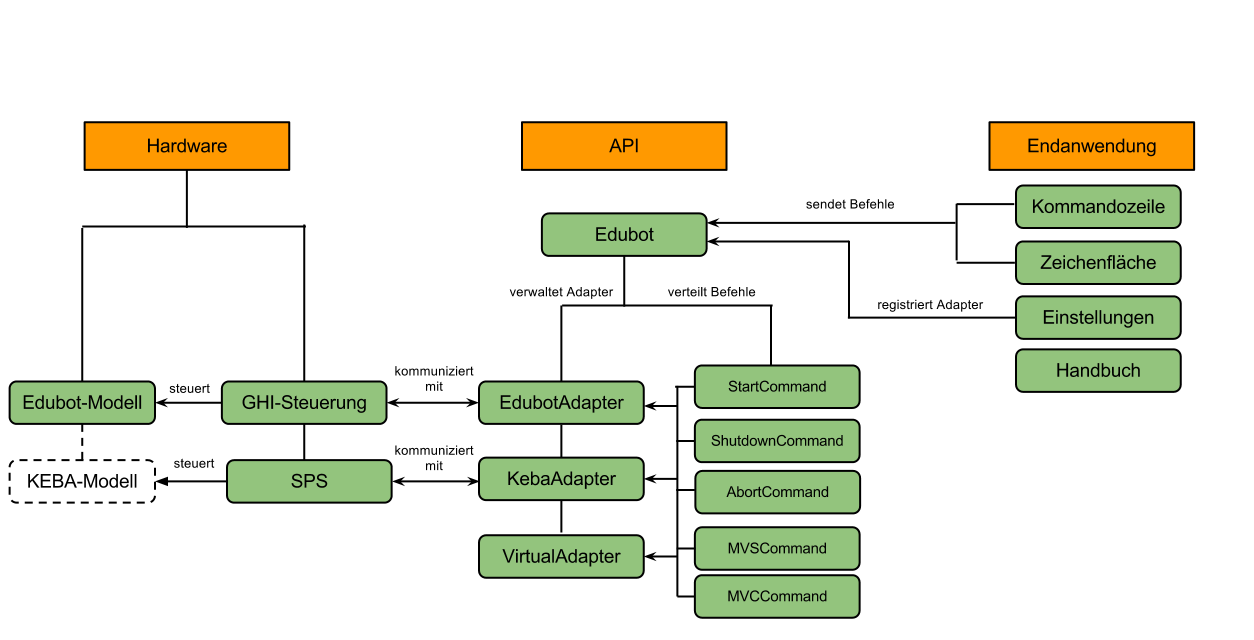
\includegraphics[width=12cm]{images/EdubotSystem} 
    \caption{Gesamtkonzept}
  \end{minipage}
\end{figure}
Die Folgende Aufzählung soll die Augabenstellungen der oben genannten Komponenten genauer erklären:
\subsubsection{Anwendung}
Die Edubot Endanwendung soll dem Benutzer eine Oberfläche bieten, welche ihm, über den Umweg der API, den Zugriff auf die Hardware ermöglicht. Die Anwendung soll über folgende Grundfunktionen verfügen:
\begin{itemize}
\item \textbf{Einstellungen}\\
Ein Berreich zur Vornahme von Einstellungen solle es ermöglichen auszuwählen ob und auf welcher Hardware eingegebene Befehle ausgegeben werden sollen. Zusätzlich soll in den Einstellungen die Konfiguraiton der benötigten Verbindungsparamter möglich sein. Ebenfalls in diesem Berreich sollen sich verschiedene Konfigurationsparameter für die Visualisierung anpassen lassen.
\item \textbf{Visualisierung}\\
Da die Software auch ohne das Anschließen von Hardware benutzbar sein soll, soll eine Simulation eines Roboters verfügbar sein. Es soll hier verschiedene Ansichten auf den Roboter geben. Die Visualisierung soll es ermöglichen sämtliche eingegebene Befehle unabhängig von der Hardware anhand eines 3D Modells eines Roboters zu Simulieren. Durch diese Funktion soll es einer größeren Anzahl von Schülern ermöglicht werden gleichzeitig mit der Software zu arbeiten.
\item \textbf{Zeichenfläche}\\
Die Endanwendung soll eine einfache Zeichenfläche bieten auf welcher der Benutzer simple Standardformen und Freihandlinien zeichnen kann. Die gezeichneten Formen werden beim drücken eines entprechenden Buttons entsprechend umgerechnet und schließlich an die API übergeben
\item \textbf{Kommandozeile}\\
Ein Kommandozeilen Tool soll es ermöglichen einzelne Befehle in einer einfachen Script Sprache einzugeben und auszuführen.
\item \textbf{Handbuch}\\
Die Anwendersoftware soll einen eigenen Berreich für die Anzeige eines Handbuches bieten. Das zur verfügung gestellte Handbuch soll nicht nur einen groben Überblick über die Funktionsweise der Anwendung geben, sondern vielmehr einen erweiterten Einblick in die Funktionsweise aller Teilberreiche diese Projekts bieten. Es soll dem Leser ermöglicht werden mehr über Robotik und den Aufbau eines einfachen Roboters zu erfahren und die zur Verfügung gestellte API zu nutzen.
\end{itemize}
\subsubsection{Hardwareinterface - API}
Eine Programmierschnittstelle ein Form einer als .dll einbindbaren dll soll alle wesentlichen Aufgaben übernehmen die zum Betrieb des Roboters nötig sind. Eine Anwendung die den Roboter benutzen will soll nur noch die eintsprechenden Funktionenen der API aufrufen müssen. Die von der API zu übernehmenden Aufgaben sind vor allem:
\begin{itemize}
\item \textbf{Invers Kinemematik}\\
Das Hardwareinterface soll die Aufgabe der Berrechnung aller Motorbewegungen übernehmen können welche zum erreichen eines Punktes nötig sind.
\item \textbf{Interpolation}\\
Es soll durch Aufruf der Entsprechenden Funktionen möglich sein, alle Punkte berrechnen zu lassen die nötig sind um eine bestimmte Form (z.B.: Kreis, Linie) zu fahren.
\item \textbf{Kommunikation mit dem Roboter}\\
Ebenfalls Aufgabe der Hardwareschnittstelle ist es, die Kommunikation mit dem Roboter über Netzwerk aufzubauen und zu verwalten, die ensprechenden Parameter für die Verbindung kommen hierfür von der die API benutzenden Anwendung. Für die Kommunikation mit dem Roboter muss ein entsprechendes Ereignissystem zur Verfügung gestellt werden, dass Ereignisse und Befehle an den Roboter schicken kann und Rückmeldungen verarbeitet.
\item \textbf{Kommunikation mit der Endanwendung}\\
Einer Anwendung welche die API verwendet, soll ausreichend Rückmeldung über den Status der Roboter und der Verbindung gegeben werden. Ebenfalls notwendig ist es, die Ergebnisse der Berechnungen and die Anwendung übergeben zu können, um beispielsweise eine Animation zu betreiben die den Roboter visualisiert.
\end{itemize}
\subsubsection{Hardware}
Im Bereich der Hardware ergeben sich zwei verschiedene, von einander nur lose abhängige Teilaufgaben:
\begin{itemize}
\item \textbf{KEBA Komponenten}\\
Von der Firma KEBA zur Verfügung gestellte Komponenten sollen bei Abschluss dieses Projektes so weit programmiert und vorbereitet sein, dass der problemlose Einbau in eine nach Abschluss des Projektes eventuell im Rahmen eines weiteren Projektes zu erstellende Mechanik gewährleistet ist. Zu diesem Zweck muss sowohl eine Netzwerkschnittstelle auf der SPS, als auch eine Anbindung für die Motoren implementiert sein. Weiters muss für die richtige Nutzung der durch die SPS zur Verfügung gestellten Grundbewegungen gesorgt werden.
Als weiterer Punkt soll eine die Grobplanung, der Teile der Alumechanik, sowie die Konstruktion der Einzelteile in Form von CNC Programmen vorhanden sein.
\item \textbf{Edubot Modell}\\
Unter dem Namen "'Edubot Model"' soll ein eigenständiger über die Netzwerkschnittstelle ansteuerbarer Roboter aus Holz zur Verfügung gestellt werden. Dieser Roboter soll von der Software kommende Befehle Ausführen und die entsprechenden Bewegungen Ausführen. Um die Aufgabenstellung dieser Komponente genauer beschreiben zu können ist sie hier zusätzlich unterteilt:
\begin{itemize}
\item \textbf{Steuerung}\\
Als Taktgeber für die Beiden Schrittmotoren soll ein Microcontroller, welcher im Laufe des Projektes ausgewählt und beschafft werden muss, dienen. Dieser Mikrocontroller soll über eine Netzwerkverbindung die benötigten Informationen von der auf dem PC laufenden Anwendung zugesant bekommen.
Auf dem Mikrocontroller soll sowohl die Synchronisation der beiden Achsen, als auch die Berechnung der benötigten Anfahr- und Bremsrampen durchgeführt werden. Der Mikrocontroller soll außerdem die Verwaltung der Motoren, sowie die Ansteuerung der Funktionen der Motorsteuerung (Nanotec SMC11) übernehmen und damit die Schnittstelle zwischen dem PC und den Motoren bilden.
\item \textbf{Mechanik und Elektronik}\\
Die Mechanik und Elektronik soll auf Basis zweier Nanotech st2818 Schrittmotoren, den dazugehörigen SMC11 Steuerung und der zugehörigen Spannungsversorgung ein funktionsfähiger Roboter erstellt werden. Dieser Roboter soll über zwei horizontale Achsen verfügen und aus einem geeigneten Werkstoff bestehen. Als Werkzeug soll am Ende der vorderen Achse ein Stift oder etwas vergleichbares montiert werden können, um das Zeichnen eines von der Anwendung vorgegebenen Weges innerhalb des Bewegungsspielraums zu ermöglichen. Die Achslängen sollen sich in Abhängigkeit von der Leistungsfähigkeit der Motoren im Bereich zwischen 15 cm und 25 cm Bewegen.
\end{itemize}  
\end{itemize}  

 


